\documentclass[11pt]{beamer}
\usepackage[utf8]{inputenc}
\usepackage[T1]{fontenc}
\usepackage{lmodern}
\usepackage{graphicx}
\usetheme{Madrid}
\begin{document}
	\author{Daniel Walther Berns}
	\title{Como usar pythonanywhere.com}
	\subtitle{con git y python}
	%\logo{}
	\institute{DIE - Facultad de Ingeniería - UNPSJB}
	\date{}
	%\subject{}
	\setbeamercovered{transparent}
	\setbeamertemplate{navigation symbols}{}
	\begin{frame}[plain]
		\maketitle
	\end{frame}
	
	\begin{frame}[fragile]
		\frametitle{PythonAnyWhere}
		
		\begin{enumerate}
		\item Se supone que la cuenta de usario en \verb-pythonanywhere.com- ya fue creada.
		
		\item Una vez que nos hemos conectado (logueado) al sitio, debemos estar viendo una pantalla llamada dashboard.
		
		\end{enumerate}
	\end{frame}

\begin{frame}
	\frametitle{Pantalla dashboard}
\begin{figure}
	\centering
	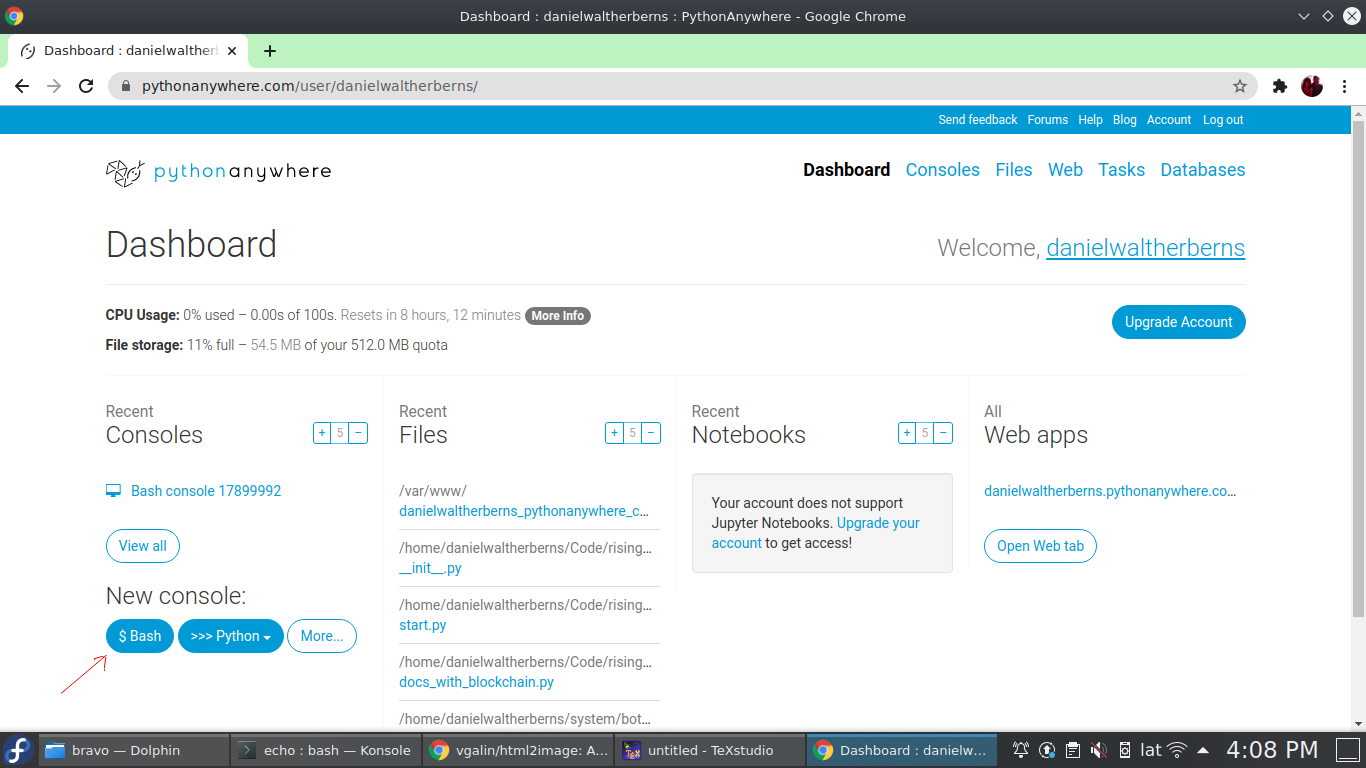
\includegraphics[width=0.7\linewidth]{sc/dashboard.png}
	\caption{Dashboard: abajo a la izquierda aparece el botón para crear una consola con Bash.}
	\label{fig:dashboard}
\end{figure}
\end{frame}

\begin{frame}[fragile]
	\frametitle{Consola con bash}
\begin{figure}
	\centering
	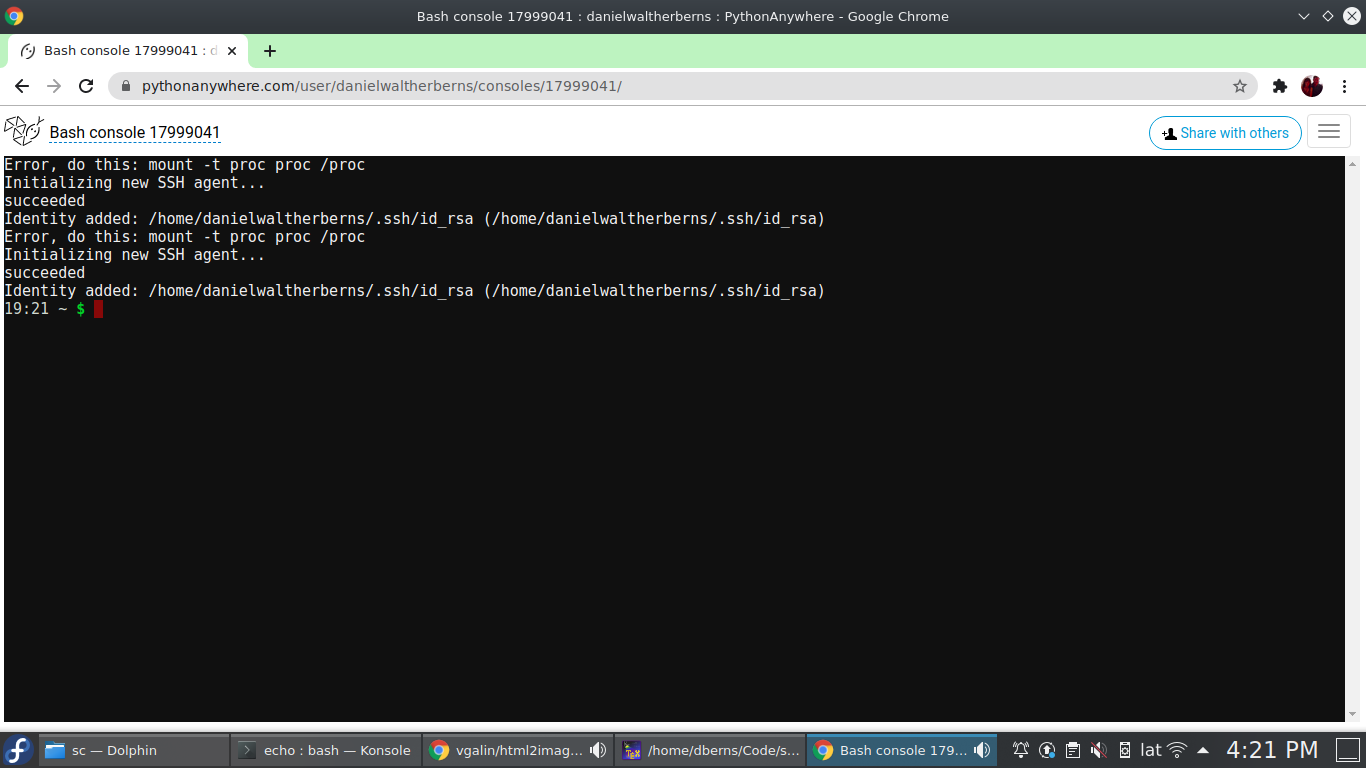
\includegraphics[width=0.7\linewidth]{sc/bash.png}
	\caption{Consola para enviar comandos a una máquina virtual con linux.}
	\label{fig:bash}
\end{figure}

\end{frame}

\begin{frame}[fragile]
	\frametitle{Comandos para trabajar en la consola}
	
\begin{enumerate}
	\item \begin{verbatim}ls\end{verbatim} para ver los archivos en el directorio actual.
	\item \begin{verbatim}pwd\end{verbatim} para ver el path o camino del directorio actual.
	\item \begin{verbatim}mkdir xyz\end{verbatim} para crear un directorio de nombre xyz.
	\item \begin{verbatim}cd xyz\end{verbatim} para moverse al directorio de nobre xyz.
\end{enumerate}
\end{frame}

\begin{frame}[fragile]
	\frametitle{Como trabajar con git}
	
\begin{enumerate}
	\item Escribimos programas en nuestras computadoras, con un entorno de programación cómodo y amigable.
	\item ``Depositamos" los programas que escribimos en un repositorio en Github.
	\item Empleamos los comandos en la consola
	\begin{verbatim}
		git clone https://github.com/usuario/repositorio.git
	\end{verbatim}
    y
	\begin{verbatim}
	git pull
    \end{verbatim}
    para transferir los programas a \verb-pythonanywhere.com-.
	
\end{enumerate}
\end{frame}

\begin{frame}
	\frametitle{Ejemplo git clone}
	\begin{figure}
		\centering
		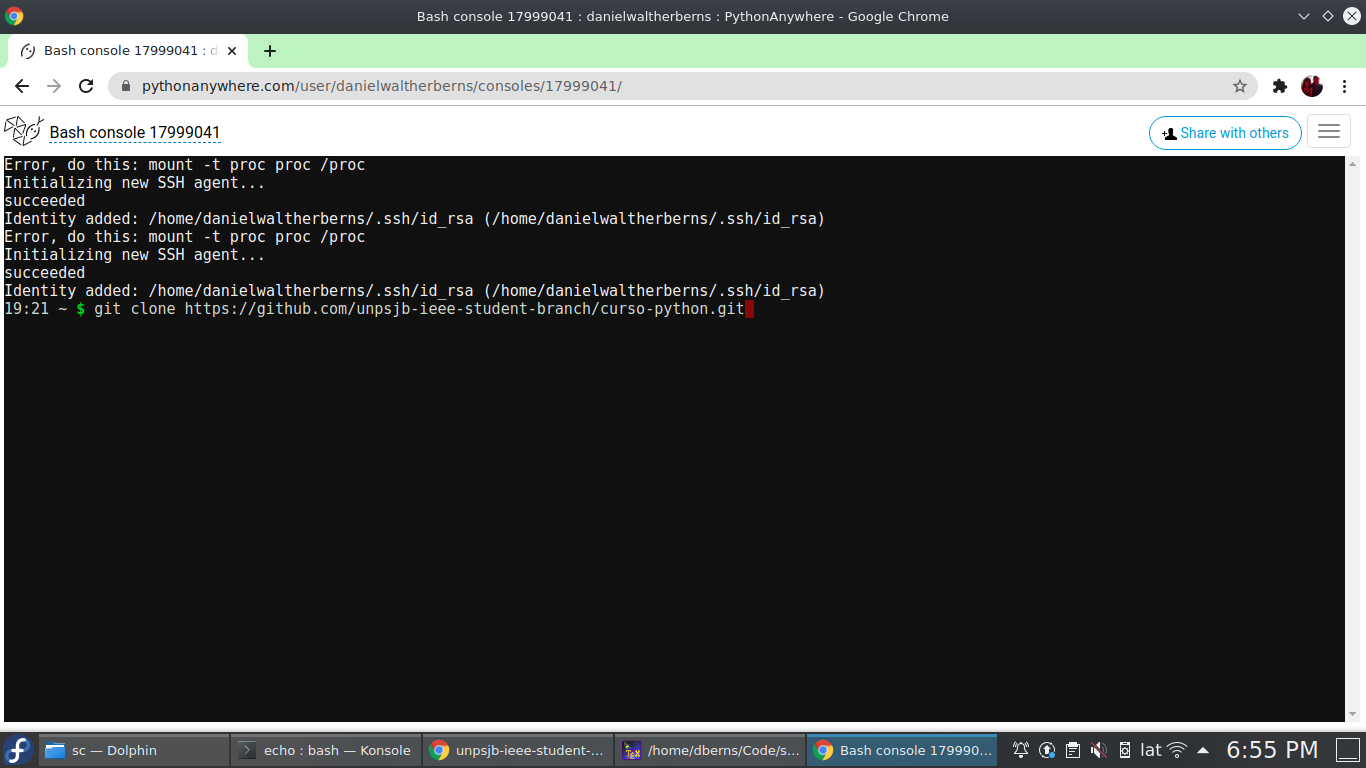
\includegraphics[width=0.7\linewidth]{sc/git_alpha}
		\caption{Antes de ejecutar git clone}
	\end{figure}
	
\end{frame}

\begin{frame}
	\frametitle{Ejemplo git clone}
	\begin{figure}
		\centering
		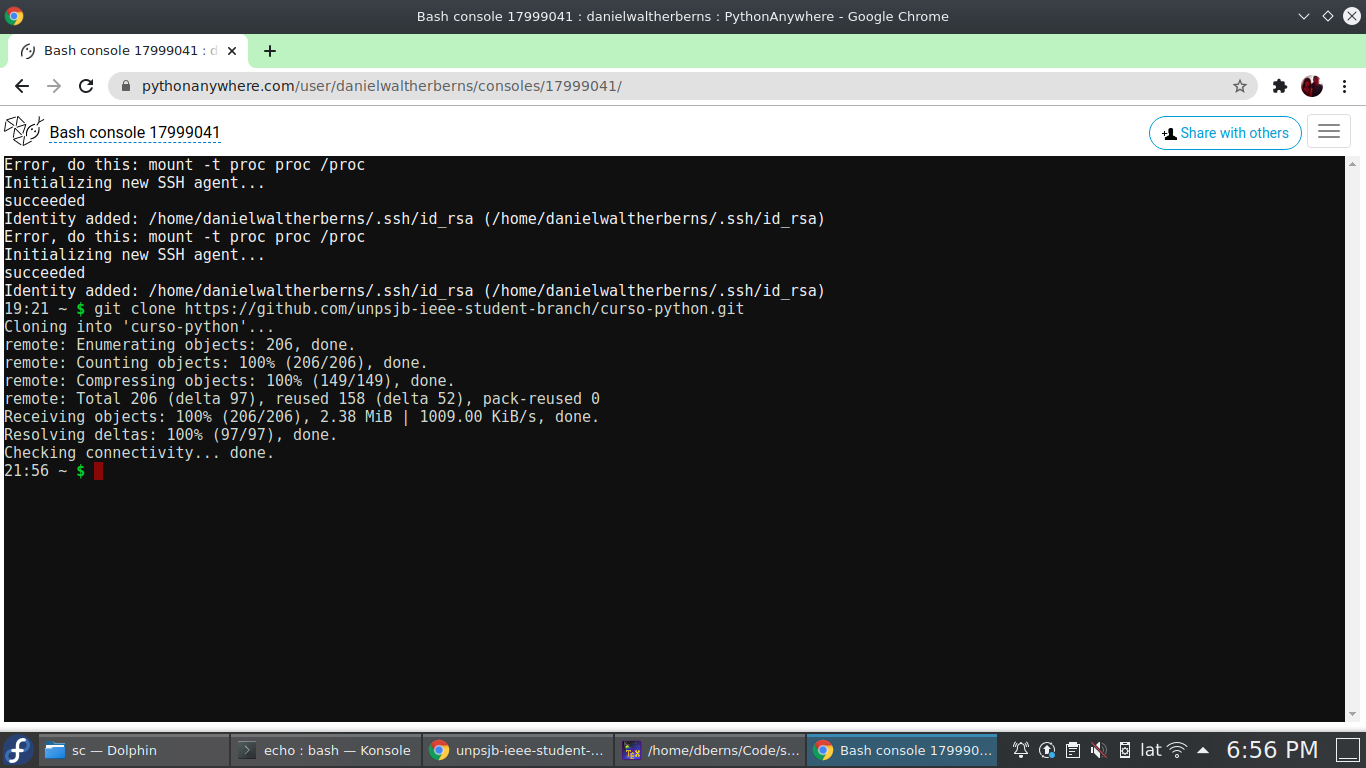
\includegraphics[width=0.7\linewidth]{sc/git_bravo}
		\caption{Resultado de ejecutar git clone}
	\end{figure}
	
\end{frame}

\begin{frame}
	\frametitle{Ejemplo cd y pwd}
	\begin{figure}
		\centering
		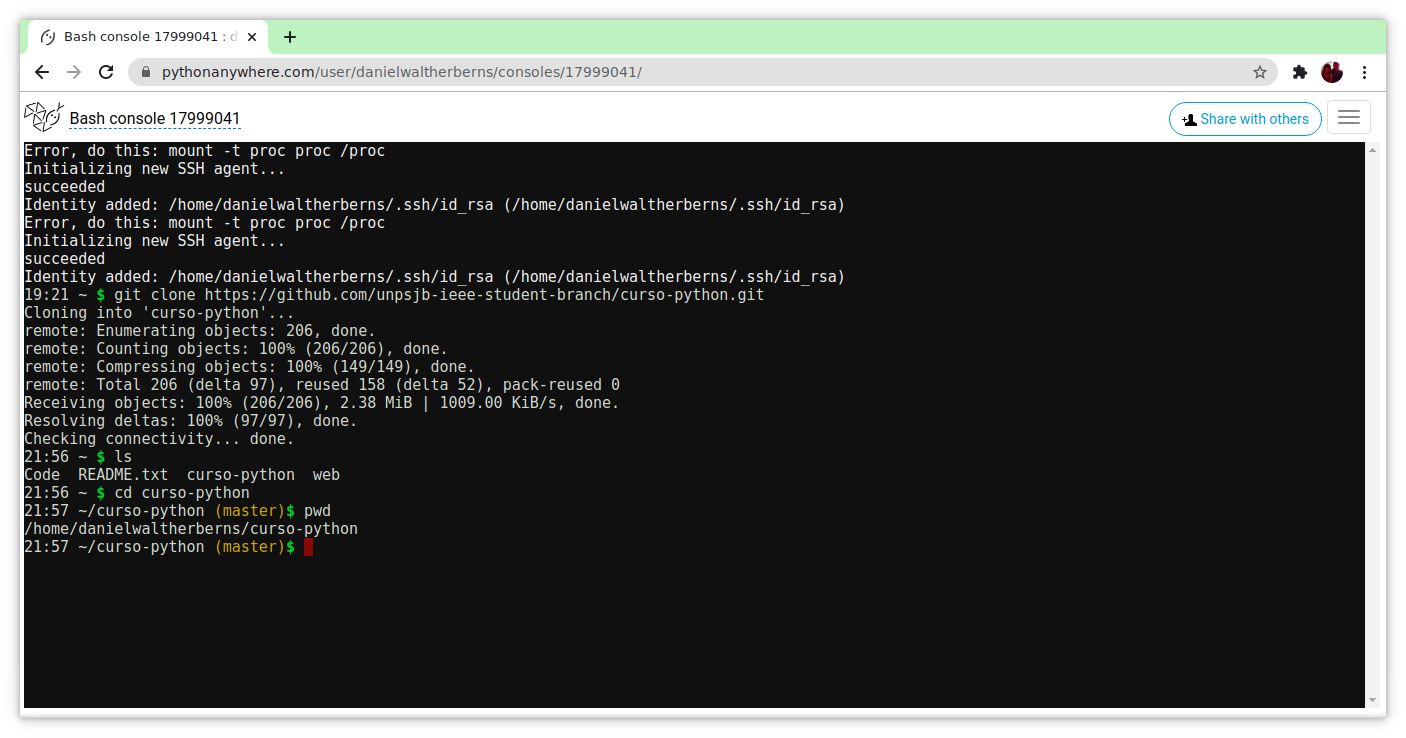
\includegraphics[width=0.7\linewidth]{sc/git_charlie}
		\caption{Resultado de ejecutar cd y pwd}
	\end{figure}
	
\end{frame}

\begin{frame}
	\frametitle{Ejemplo ls}
	\begin{figure}
		\centering
		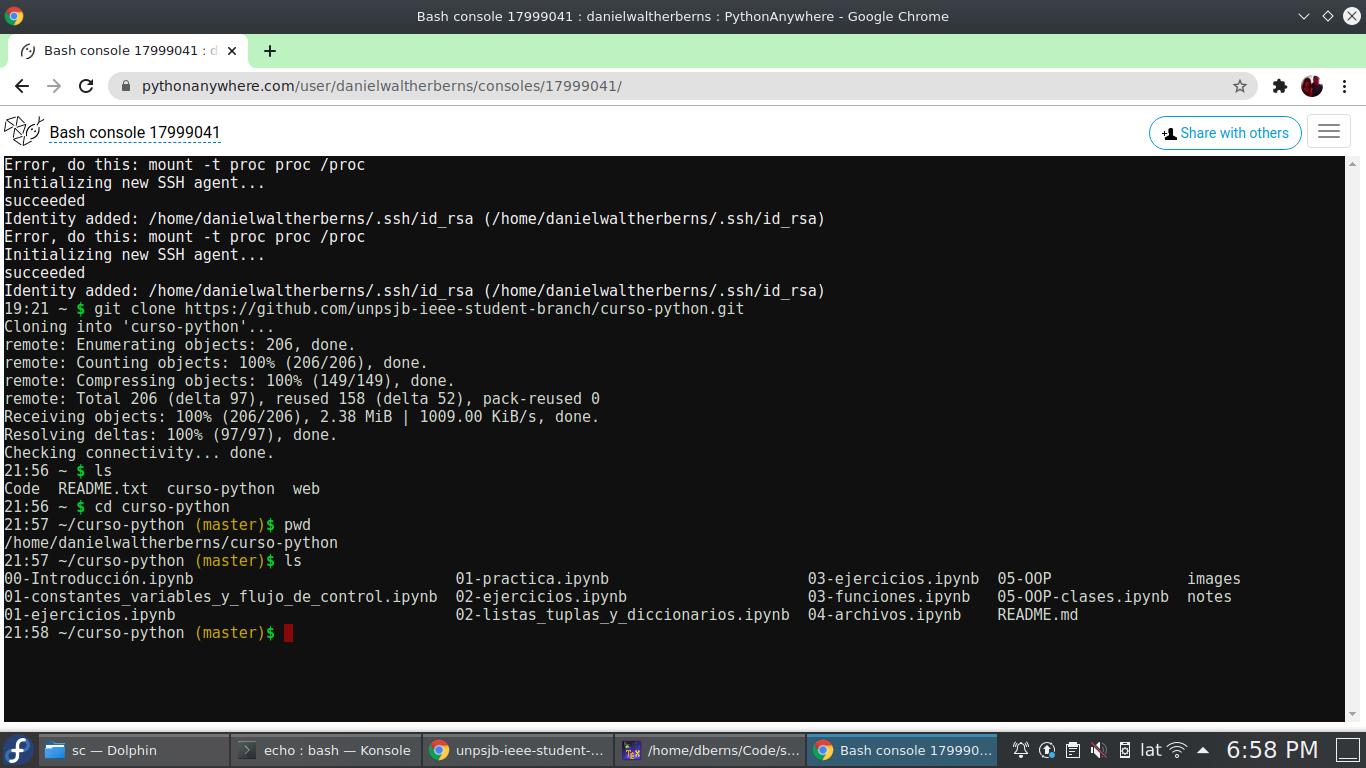
\includegraphics[width=0.7\linewidth]{sc/git_delta}
		\caption{Resultado de ejecutar cd y pwd}
	\end{figure}
	
\end{frame}

\begin{frame}
	\frametitle{Como ejecutar python en la consola de pythonanywhere}
	\begin{figure}
		\centering
		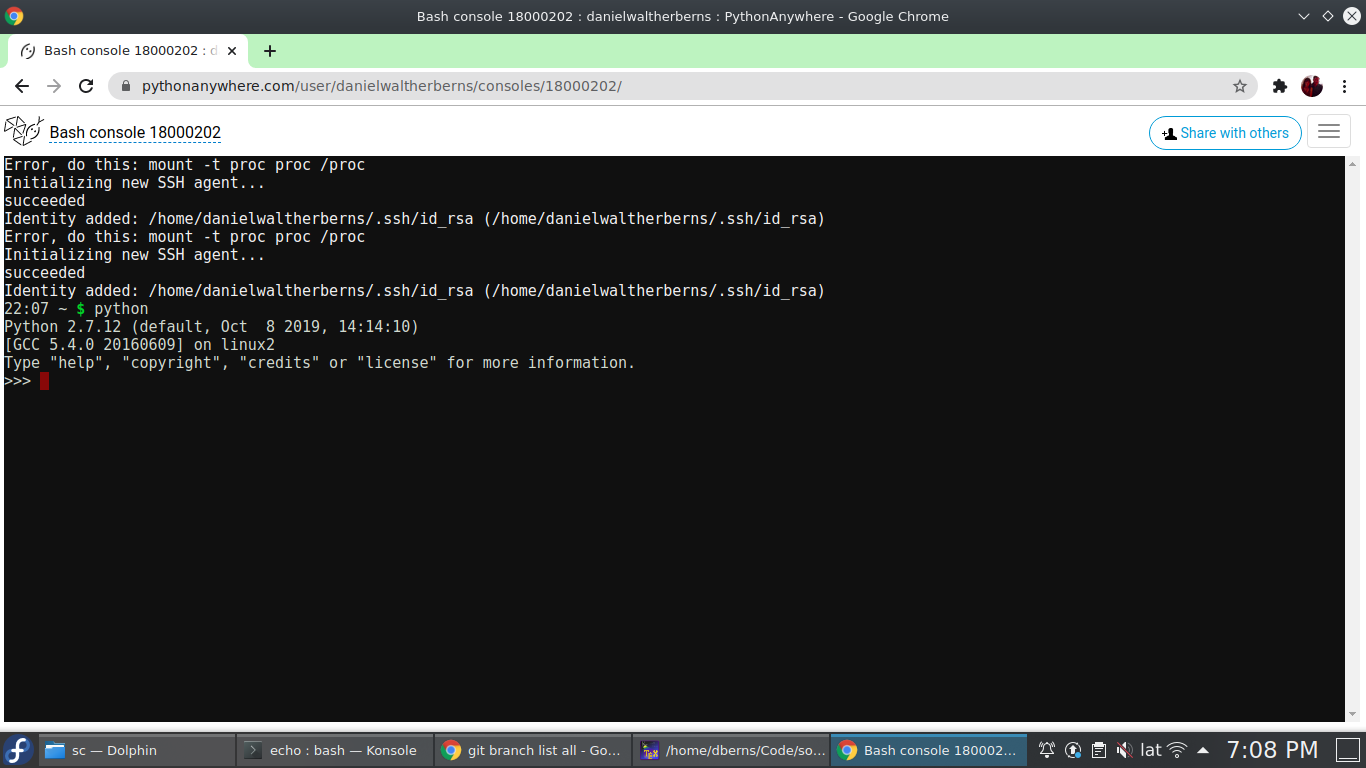
\includegraphics[width=0.7\linewidth]{sc/bash_python_2}
		\caption{Python 2: este NO!}
	\end{figure}
	
\end{frame}

\begin{frame}
	\frametitle{Como ejecutar python en la consola de pythonanywhere}
	\begin{figure}
		\centering
		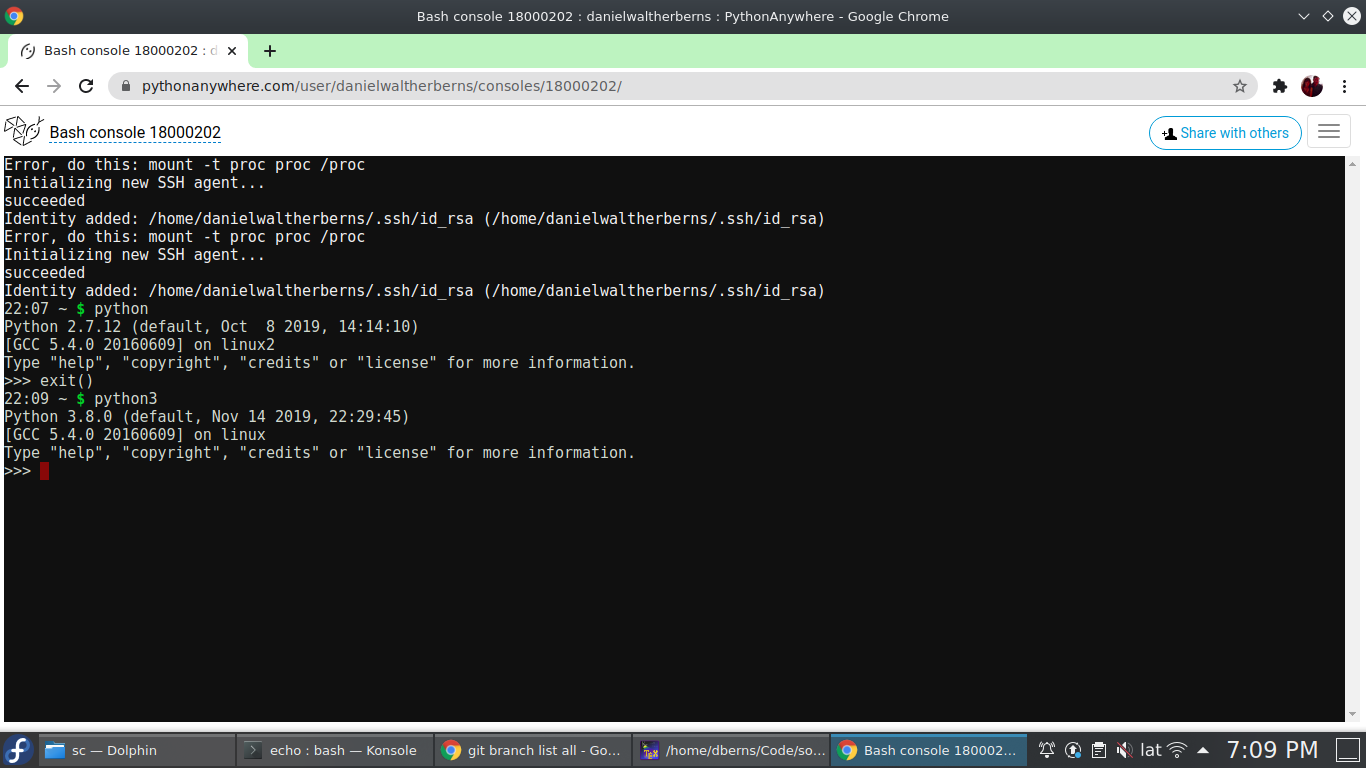
\includegraphics[width=0.7\linewidth]{sc/bash_python_3}
		\caption{Python 3: este SI!}
	\end{figure}
	
\end{frame}

\begin{frame}
	\frametitle{Como salir de la consola}
	\begin{figure}
		\centering
		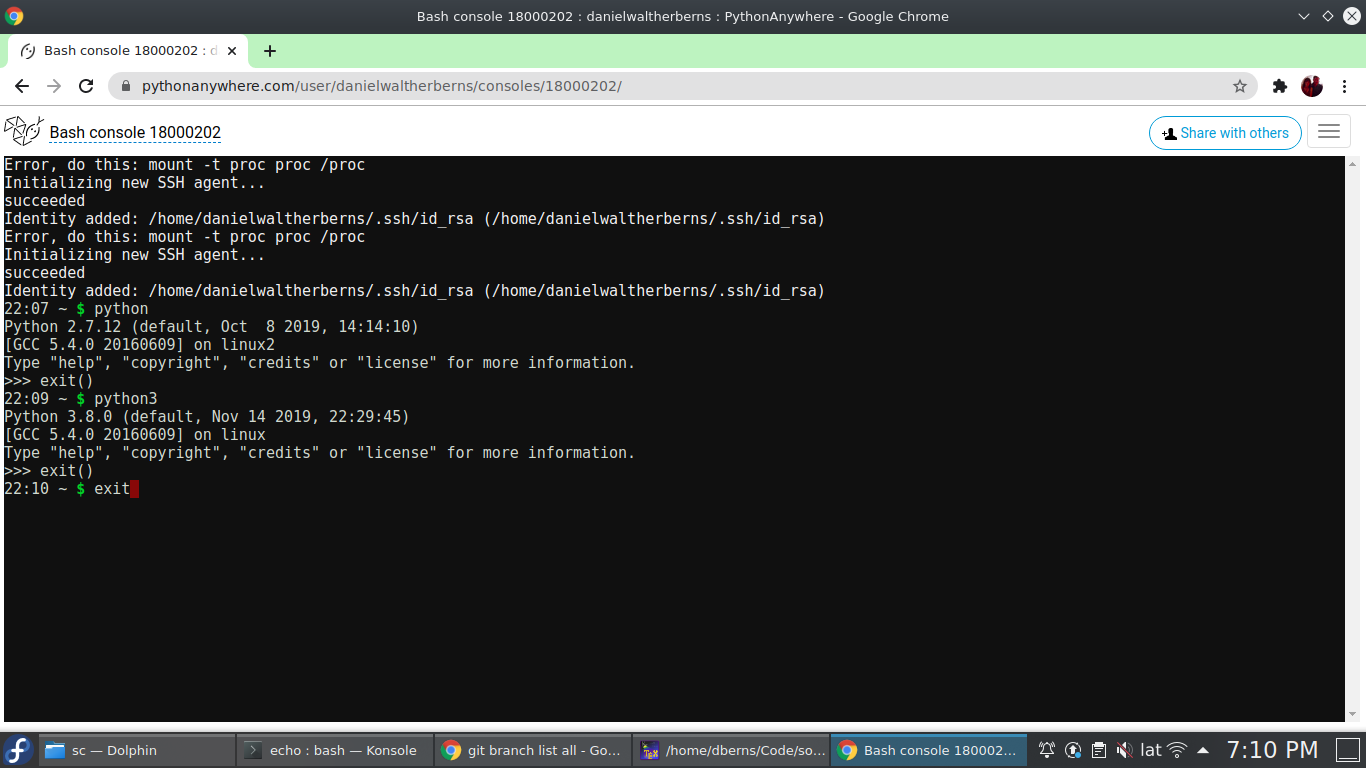
\includegraphics[width=0.7\linewidth]{sc/bash_exit}
		\caption{comando exit en la consola, para cerrarla.}
	\end{figure}
	
\end{frame}

\end{document}